%%%%%%%%%%%%%%%%%%%%%%%%%%%%%%%%%%%%%%%%%
% agent-spec-kit — MEng Final Presentation
% Imperial College London beamer theme
%
%!TEX program = xelatex
% Must be compiled with XeLaTeX (custom Imperial Sans fonts).
%%%%%%%%%%%%%%%%%%%%%%%%%%%%%%%%%%%%%%%%%

\documentclass[
	aspectratio=169, % 16:9
	t,               % top-align content
	onlytextwidth,
	10pt,
]{beamer}

\usetheme{Imperial}

% Look for images in images/ (theme default is Images/)
\graphicspath{{images/}{./}}

%----------------------------------------------------------------------------------------
%	PACKAGES
%----------------------------------------------------------------------------------------
\usepackage{tikz}
\usetikzlibrary{arrows.meta, positioning, shapes.geometric, fit, backgrounds}
\usepackage{listings}
\usepackage{pgfplots}
\pgfplotsset{compat=1.17}

% Code listing style (kept short; uses the document sans/mono fonts)
\definecolor{codebg}{RGB}{245,245,250}
\definecolor{codekw}{RGB}{0,0,160}
\definecolor{codecm}{RGB}{120,120,130}
\definecolor{codestr}{RGB}{0,120,90}
\lstset{
	language=Python,
	basicstyle=\ttfamily\scriptsize,
	backgroundcolor=\color{codebg},
	keywordstyle=\color{codekw}\bfseries,
	commentstyle=\color{codecm}\itshape,
	stringstyle=\color{codestr},
	morekeywords={async,await,scenario,fixture},
	showstringspaces=false,
	breaklines=true,
	columns=fullflexible,
	frame=single,
	rulecolor=\color{ICLBlue!30},
	framesep=6pt,
	xleftmargin=4pt,
	xrightmargin=4pt,
	aboveskip=4pt,
	belowskip=2pt,
}

% Re-usable TikZ node styles for the architecture diagram
\tikzset{
	flow/.style={rectangle, rounded corners=2pt, draw=ICLBlue, line width=0.6pt,
		fill=ICLBlue!8, text=ICLBlue, font=\scriptsize\bfseries,
		minimum height=8mm, minimum width=20mm, align=center, inner sep=3pt},
	store/.style={flow, draw=ICLDarkBlue, fill=ICLLightGrey, text=ICLDarkBlue},
	fail/.style={flow, draw=red!60!black, fill=red!6, text=red!60!black},
	arr/.style={-{Stealth[length=2mm]}, line width=0.6pt, draw=ICLBlue!70},
}

% Small helpers for oracle "chips"
\newcommand{\chip}[2]{\tikz[baseline=(c.base)]{\node[fill=#1,text=white,rounded corners=2pt,
	font=\scriptsize\bfseries,inner sep=2.2pt] (c) {#2};}}
\newcommand{\Ochip}{\chip{ICLBlue}{\,O\,}}
\newcommand{\Tchip}{\chip{ICLBlue!70}{\,T\,}}
\newcommand{\Schip}{\chip{ICLDarkBlue}{\,S\,}}

%----------------------------------------------------------------------------------------
%	PRESENTATION INFORMATION
%----------------------------------------------------------------------------------------
\title{agent-spec-kit}
\subtitle{Scenario-Driven Evaluation and Testing of Tool-Using LLM Agents}
\author{Ruthvik Konduru}
\date{June 2026}

\begin{document}

%----------------------------------------------------------------------------------------
%	TITLE SLIDE  (logo-led, white background)
%----------------------------------------------------------------------------------------
\begingroup
	\setbeamercolor{title page title}{fg=ICLBlue}
	\setbeamercolor{title page subtitle}{fg=ICLBlue}
	\setbeamercolor{author}{fg=ICLBlue}
	\setbeamercolor{date}{fg=ICLBlue}
	\setbeamertemplate{title page}[logo]{imperial_logo.png}
	\frame[plain, s]{\titlepage}
\endgroup

%----------------------------------------------------------------------------------------
%	1. MOTIVATION
%----------------------------------------------------------------------------------------
\begin{frame}
	\frametitle{Tool-using agents act on the world}
	\begin{columns}[T]
		\begin{column}{0.5\linewidth}
			\begin{itemize}
				\setlength\itemsep{0.8em}
				\item LLMs are no longer just text generators --- as \textbf{agents} they
				plan, call tools, and \textbf{change external state}.
				\item Correctness can therefore \textbf{not} be judged from the final reply alone.
				\item A support agent can sound perfectly polite while it:
				\begin{itemize}
					\setlength\itemsep{0.3em}
					\item skips \textbf{authentication} and leaks account data,
					\item calls the \textbf{wrong tool} or in the wrong order,
					\item leaves the \textbf{database} in an invalid state.
				\end{itemize}
			\end{itemize}
			\vspace{0.4em}
			{\footnotesize\textcolor{ICLBlue}{The plausible answer is only \emph{one} part of being correct.}}
		\end{column}
		\begin{column}{0.48\linewidth}
			\centering
			\vspace{0.2em}
			\scalebox{1.18}{%
			\begin{tikzpicture}[font=\scriptsize,
				good/.style={draw=green!55!black, fill=green!8, rounded corners=3pt, inner sep=4pt},
				bad/.style={draw=red!65!black, fill=red!6, rounded corners=3pt, inner sep=4pt},
				lbl/.style={font=\tiny, text=ICLBlue}]
				% agent
				\node[flow, minimum width=20mm] (ag) {Support agent};
				% the visible reply -- looks great
				\node[good, right=10mm of ag, text width=24mm, align=left] (reply)
					{``Done --- your refund is\\sorted, have a great day!''\ \textcolor{green!55!black}{\ding{52}}};
				\node[lbl, above=1pt of reply] {\Ochip\ \textbf{reply} (looks fine)};
				% hidden trace -- wrong
				\node[bad, below=8mm of reply, text width=24mm, align=left] (trace)
					{\texttt{get\_account()} \textcolor{red!65!black}{\ding{56}}\\\scriptsize\emph{before} \texttt{authenticate()}};
				% hidden state -- wrong
				\node[bad, below=6mm of trace, text width=24mm, align=left] (state)
					{ticket left \texttt{OPEN} \textcolor{red!65!black}{\ding{56}}\\\scriptsize refund never written};
				% arrows first, then labels sit cleanly on top
				\draw[arr] (ag) -- (reply);
				\draw[arr, draw=red!55!black] (ag.south) |- (trace.west);
				\draw[arr, draw=red!55!black] (ag.south) |- (state.west);
				\node[lbl, fill=white, inner sep=1.5pt, align=center, left=6mm of trace]
					{\Tchip\\[2pt]wrong order};
				\node[lbl, fill=white, inner sep=1.5pt, align=center, left=6mm of state]
					{\Schip\\[2pt]bad state};
			\end{tikzpicture}}\\[6pt]
			{\footnotesize\textcolor{ICLBlue}{The reply passes; the actions and state silently do not.}}
		\end{column}
	\end{columns}
\end{frame}

%------------------------------------------------
\begin{frame}
	\frametitle{Correctness lives on three surfaces}
	\framesubtitle{Output is necessary but far from sufficient}

	\vspace{1.2em}
	\begin{columns}[T,onlytextwidth]
		\begin{column}{0.3\linewidth}
			\centering
			\tikz\node[rounded corners=4pt, fill=ICLBlue, text=white, minimum width=3cm,
				minimum height=1.7cm, font=\fontsize{34}{34}\selectfont\bfseries]{O};\\[8pt]
			{\large\color{ICLBlue}\textbf{Output}}\\[2pt]
			{\footnotesize\color{ICLBlue}what the agent \emph{says}}
		\end{column}
		\hfill
		\begin{column}{0.3\linewidth}
			\centering
			\tikz\node[rounded corners=4pt, fill=ICLBlue!65, text=white, minimum width=3cm,
				minimum height=1.7cm, font=\fontsize{34}{34}\selectfont\bfseries]{T};\\[8pt]
			{\large\color{ICLBlue}\textbf{Trace}}\\[2pt]
			{\footnotesize\color{ICLBlue}which \emph{tools} it called}
		\end{column}
		\hfill
		\begin{column}{0.3\linewidth}
			\centering
			\tikz\node[rounded corners=4pt, fill=ICLDarkBlue, text=white, minimum width=3cm,
				minimum height=1.7cm, font=\fontsize{34}{34}\selectfont\bfseries]{S};\\[8pt]
			{\large\color{ICLBlue}\textbf{State}}\\[2pt]
			{\footnotesize\color{ICLBlue}the \emph{state} it left behind}
		\end{column}
	\end{columns}
	\vspace{2.2em}
	\begin{center}
		\begin{minipage}{0.78\linewidth}
			\centering\color{ICLBlue}
			A failure on \emph{any} surface can be hidden by a fluent reply ---
			and may even be masked by recovery on a later turn.
		\end{minipage}
	\end{center}
\end{frame}

%------------------------------------------------
\begin{frame}
	\frametitle{Existing tools only cover part of the loop}
	\begin{columns}[T]
		\begin{column}{0.54\linewidth}
			\begin{itemize}
				\setlength\itemsep{0.6em}
				\item \textbf{Output graders / LLM-as-judge} (HELM, G-Eval, MT-Bench): great for
				comparing models on isolated final answers --- but \emph{blind} to tool and state failures.
				\item \textbf{Agent benchmarks} ($\tau$-bench, AppWorld, WebArena): trace/state aware,
				but \emph{fixed leaderboards}, not reusable infrastructure for your own agent.
				\item \textbf{Trace viewers} (LangSmith, Langfuse): show \emph{what} happened ---
				the developer still has to infer what \emph{should} have happened.
			\end{itemize}
			\vspace{0.4em}
			\begin{block}{\small The gap}
				\small No single, reusable way to assert over \textbf{output + trace + state}
				in one multi-turn scenario --- with \textbf{precise diagnostics} when a check fails.
			\end{block}
		\end{column}
		\begin{column}{0.44\linewidth}
			\centering
			\vspace{0.1em}
			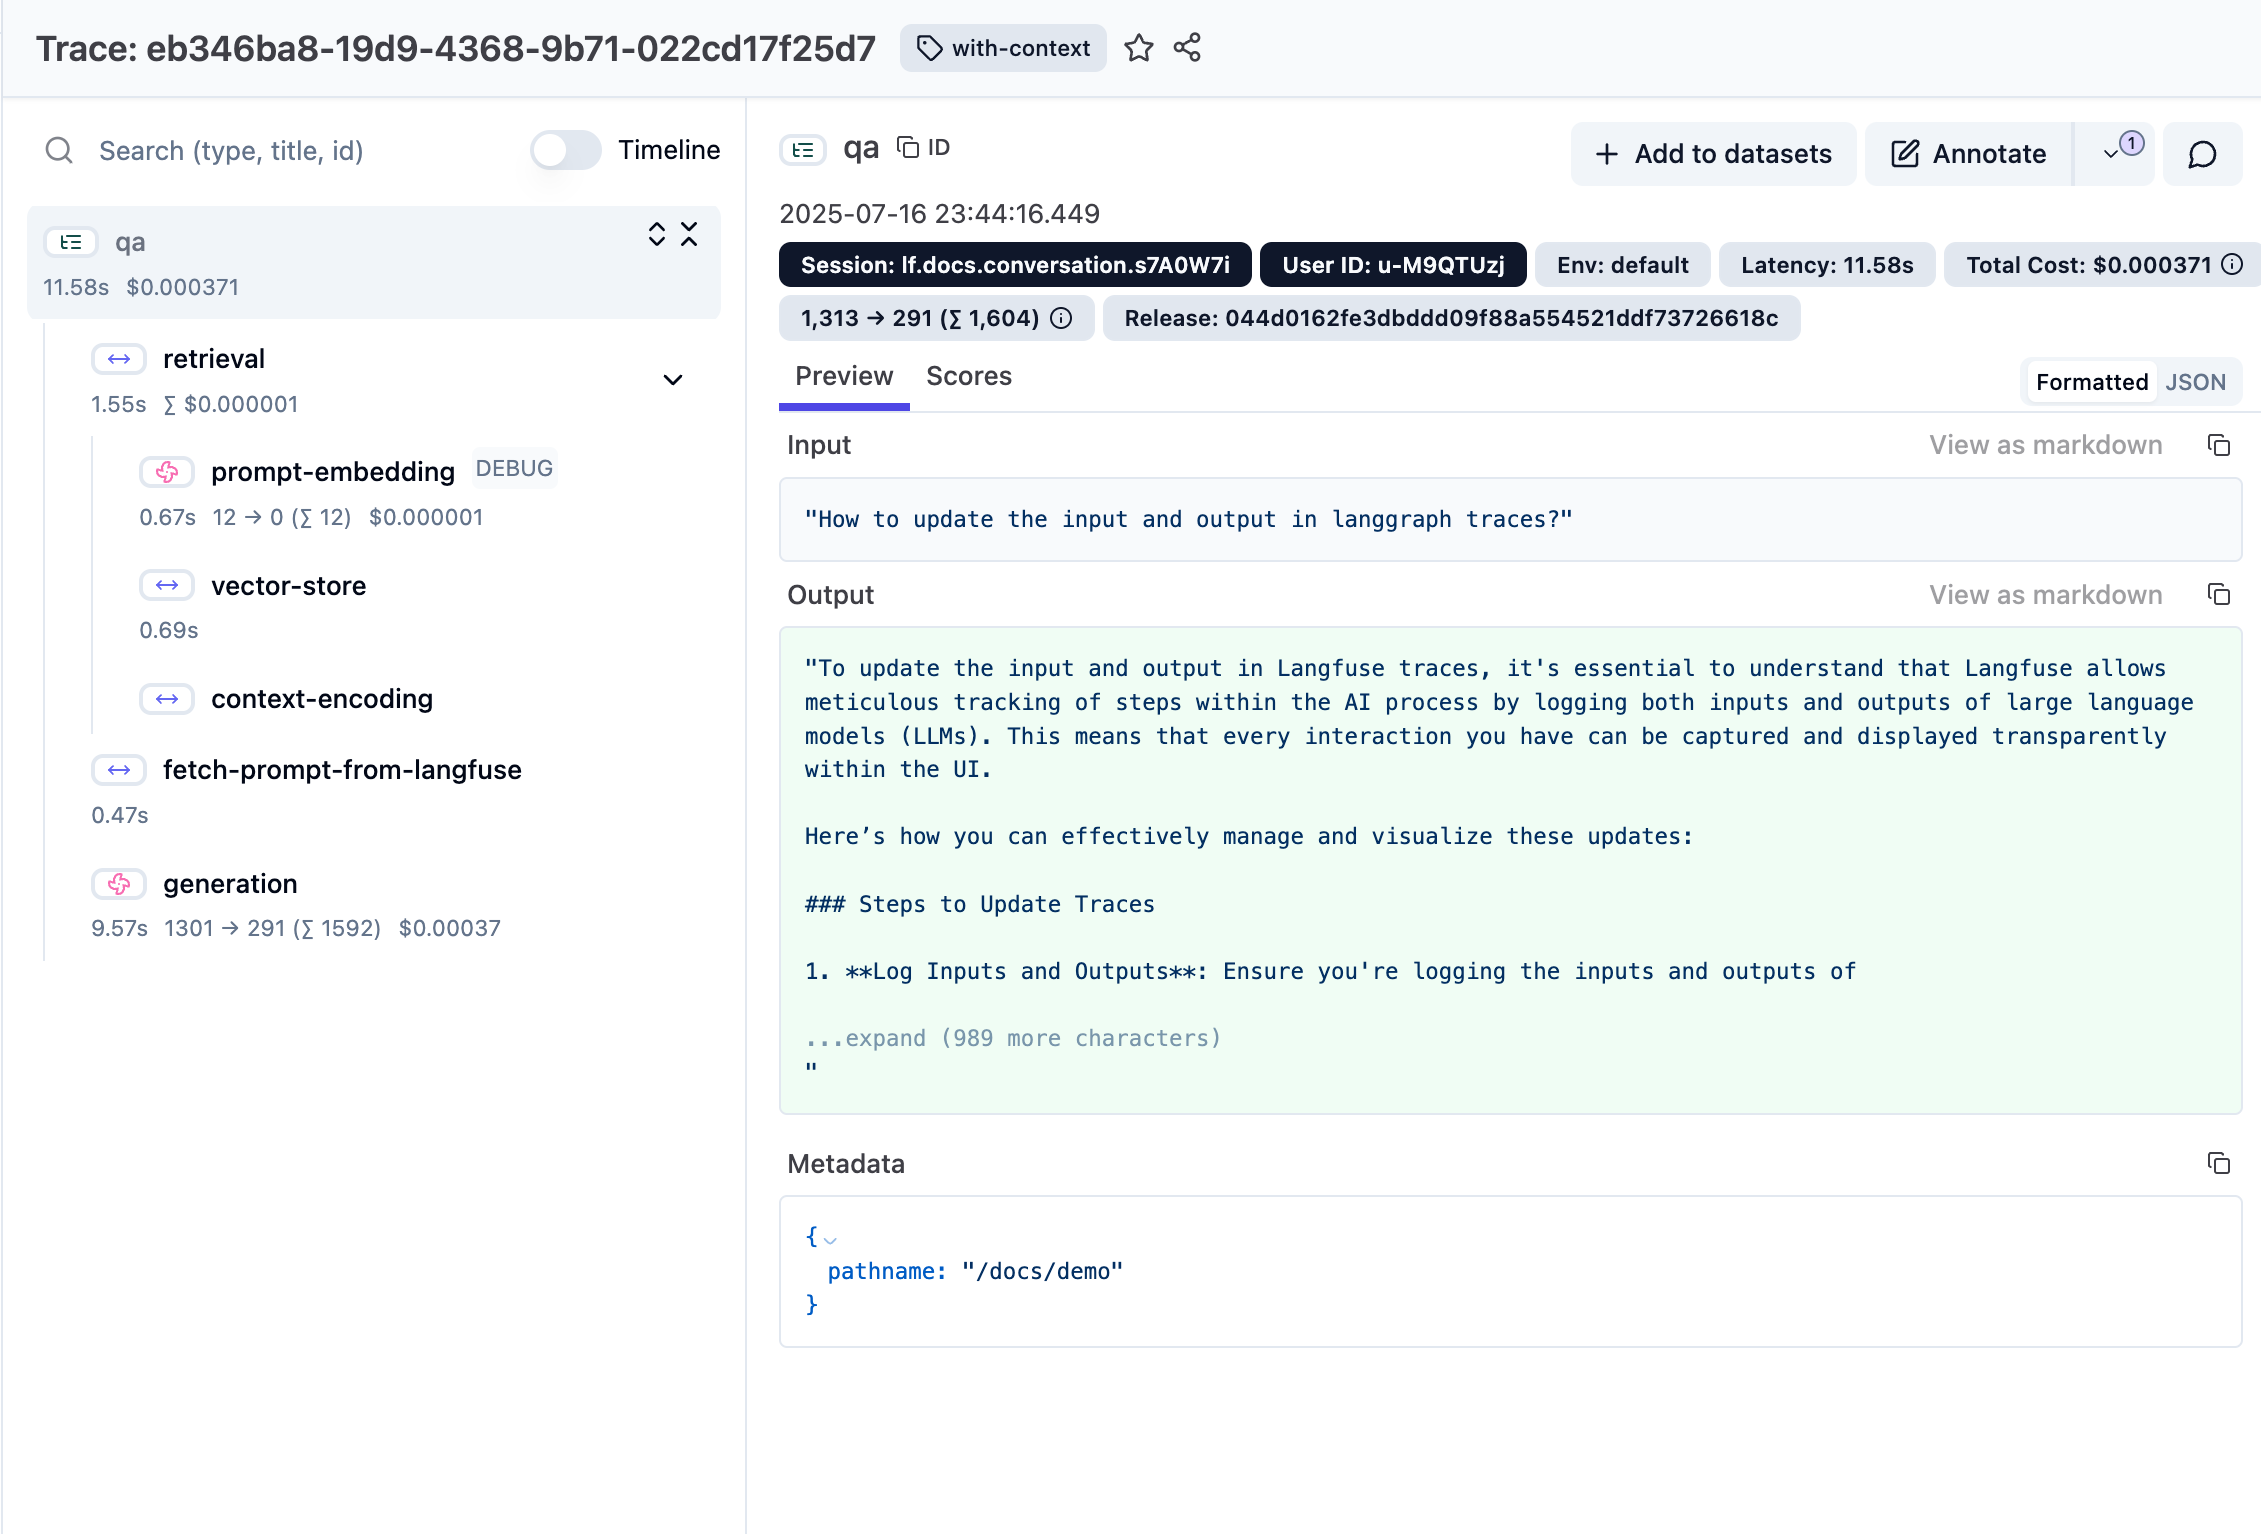
\includegraphics[width=\linewidth, height=0.66\textheight, keepaspectratio]{langfuse_example_trace.png}\\[5pt]
			{\footnotesize\textcolor{ICLBlue}{Trace viewers show the episode; they do not encode the expected behaviour.}}
		\end{column}
	\end{columns}
\end{frame}

%------------------------------------------------
\begin{frame}
	\frametitle{Research question}
	\vspace{1.0em}
	\begin{center}
	\begin{minipage}{0.86\linewidth}
		% blue accent bar + question
		\hspace{-4mm}\begin{tikzpicture}[baseline=(txt.north)]
			\node[anchor=north west, text width=0.95\linewidth, inner sep=0pt] (txt) {%
				{\Large Can the evaluation of \textbf{stateful, tool-using LLM agents} be
				expressed in a \textbf{software-testing style}:}\\[0.7em]
				{\Large readable scenarios that combine assertions over \textbf{replies},
				\textbf{tool trajectories}, and \textbf{application state}, while keeping enough
				structured evidence to \textbf{diagnose} failures precisely?}%
			};
			\draw[line width=2.2pt, ICLBlue] ([xshift=-5mm]txt.north west) -- ([xshift=-5mm]txt.south west);
		\end{tikzpicture}

		\vspace{1.6em}
		\begin{beamercolorbox}[wd=\linewidth, sep=10pt, rounded=true]{}%
			\colorbox{ICLBlue!10}{\parbox{\dimexpr\linewidth-20pt}{%
				\color{ICLBlue}\textbf{Answer:}\ \emph{agent-spec-kit} --- a scenario-driven
				testing framework for LLM agents, evaluated on a 50-task benchmark.}}
		\end{beamercolorbox}
	\end{minipage}
	\end{center}
\end{frame}

%----------------------------------------------------------------------------------------
%	SECTION DIVIDER: THE LIBRARY
%----------------------------------------------------------------------------------------
\begingroup
	\setbeamercolor{normal text}{fg=ICLBlue}\usebeamercolor[fg]{normal text}
	\setbeamercolor{page number in head/foot}{fg=white}
	\begin{frame}[plain]
		\vspace{6mm}
		\hfill
\includegraphics[width=3.2cm]{imperial_logo.png}\\[1.2cm]
		\begin{adjustwidth}{0cm}{0.15\textwidth}
			{\Huge{\ImperialSansSemiBold Part I --- The Library}}\\[0.5cm]
			{\large\ImperialSansMedium \emph{agent-spec-kit}: behaviour as executable scenarios}
		\end{adjustwidth}
	\end{frame}
\endgroup

%------------------------------------------------
\begin{frame}[fragile]
	\frametitle{The core idea: a scenario \emph{is} a conversation script}
	\framesubtitle{Output, tool, and state checks live together, woven in after each turn}

	\begin{columns}[T]
		\begin{column}{0.62\linewidth}
\begin{lstlisting}
@scenario(agent_fixture="agent", user_fixture="user")
async def test_billing_credit(s, store):
    s.user_message("I was double charged in October")
    # O: the reply must insist on verifying first
    s.assert_output(m.contains("verify"))
    # T: the agent must authenticate before account tools
    s.assert_tool_calls([
        m.tool_call("authenticate_customer"),
        m.tool_call("get_billing", args={"id": "CUST-045"}),
    ])
    # S: a postcondition on the database state
    s.assert_that(assert_credit_policy)
\end{lstlisting}
		\end{column}
		\begin{column}{0.36\linewidth}
			\begin{itemize}
				\setlength\itemsep{0.5em}
				\item \Ochip\ \texttt{assert\_output} --- the reply
				\item \Tchip\ \texttt{assert\_tool\_calls} / \texttt{forbid\_tool\_calls} --- the trace
				\item \Schip\ \texttt{assert\_that} --- environment / DB state
			\end{itemize}
			\vspace{0.4em}
			{\footnotesize One file reads like a dialogue with the contract inlined ---
			no separate datasets, graders, and runner config.}
		\end{column}
	\end{columns}
\end{frame}

%------------------------------------------------
\begin{frame}[fragile]
	\frametitle{One composable matcher language}
	\framesubtitle{Start simple: matching the reply}
	\begin{columns}[T,onlytextwidth]
		\begin{column}{0.37\linewidth}
			\begin{itemize}
				\setlength\itemsep{0.9em}
				\item Literals, \texttt{dict}s and \texttt{list}s are \emph{coerced} into matchers
				automatically.
				\item Combine them: \texttt{m.one\_of} (any), \texttt{m.all\_of} (all),
				\texttt{m.not\_}, \texttt{m.contains}, \texttt{m.regex}.
				\item Selective \textbf{LLM rubric} only where text needs judgement --- pass/fail
				criteria, not opaque scores.
			\end{itemize}
		\end{column}
		\hfill
		\begin{column}{0.55\linewidth}
\begin{lstlisting}
# deterministic: offer a refund OR a credit
s.assert_output(
  m.one_of(
    m.contains("refund"),
    m.contains("account credit"),
  )
)
\end{lstlisting}
			\vspace{0.6em}
\begin{lstlisting}
# nuance? hand that one check to an LLM judge
s.assert_output(m.llm_criteria(
  criteria=["acknowledges the double charge",
            "does not promise a refund yet"],
  threshold=2,
))
\end{lstlisting}
		\end{column}
	\end{columns}
\end{frame}

%------------------------------------------------
\begin{frame}[fragile]
	\frametitle{Matching the tool trace}
	\framesubtitle{Order and extras are explicit, not implied}
	\begin{columns}[T,onlytextwidth]
		\begin{column}{0.37\linewidth}
			\begin{itemize}
				\setlength\itemsep{0.9em}
				\item \texttt{assert\_tool\_calls} matches the \emph{normalised} tool trace.
				\item \texttt{ordered=True} pins the sequence; \texttt{ordered=False} for parallel siblings.
				\item \texttt{allow\_extras=True} lets other calls interleave; \texttt{forbid\_tool\_calls}
				asserts a tool is \emph{never} used.
			\end{itemize}
		\end{column}
		\hfill
		\begin{column}{0.55\linewidth}
\begin{lstlisting}
s.assert_tool_calls(
  [
    m.tool_call("authenticate_customer"),
    m.tool_call("get_billing",
                args={"id": "CUST-045"}),
  ],
  ordered=True,       # must appear in order
  allow_extras=True,  # others may interleave
)
\end{lstlisting}
		\end{column}
	\end{columns}
\end{frame}

%------------------------------------------------
\begin{frame}[fragile]
	\frametitle{\ldots and the matchers compose}
	\framesubtitle{Structured objects and conditional rules}
	\begin{columns}[T,onlytextwidth]
		\begin{column}{0.36\linewidth}
			\begin{itemize}
				\setlength\itemsep{0.8em}
				\item \texttt{m.object} constrains structured args or results --- only the fields
				you name.
				\item \texttt{m.list} matches sequences \texttt{ordered} or \texttt{unordered}.
				\item \textbf{Conditional rules}: \texttt{require}/\texttt{forbid} a field only
				\emph{when} another field holds.
			\end{itemize}
		\end{column}
		\hfill
		\begin{column}{0.55\linewidth}
\begin{lstlisting}
m.tool_call("open_incident", args=m.object(
  {
    "id": m.regex(r"INC-\d{4}-\d+"),
    "severity": m.one_of("high", "medium"),
    "components": m.list(["edge", "core"],
                         mode="unordered"),
  },
  rules=[                        # conditional
    m.require("pager_group")
     .when(m.field("severity") == "high"),
    m.forbid("pager_group")
     .when(m.field("severity") == "medium"),
  ],
))
\end{lstlisting}
		\end{column}
	\end{columns}
\end{frame}

%------------------------------------------------
\begin{frame}
	\frametitle{Precise diagnostics: structured counterexamples}
	\framesubtitle{When a check fails, you learn \emph{which} expectation broke, \emph{where}}
	\begin{columns}[T]
		\begin{column}{0.46\linewidth}
			\begin{itemize}
				\setlength\itemsep{0.5em}
				\item Every failed assertion produces a \textbf{Counterexample}:
				\begin{itemize}\setlength\itemsep{0.2em}
					\item headline + human location (``assert\_tool\_calls after turn \#2'')
					\item a \textbf{JSON-pointer path} to the mismatch, e.g. \texttt{\$[1].args.line\_id}
					\item expected vs.\ actual, plus a bounded event trace
				\end{itemize}
				\item Identical view in the \textbf{terminal}, the \textbf{SQLite} store, and the \textbf{web UI}.
				\item Turns ``it failed somehow'' into ``\emph{this} check broke \emph{here}''.
			\end{itemize}
		\end{column}
		\begin{column}{0.52\linewidth}
			\centering
			\vspace{0.2em}
			\begin{tikzpicture}[font=\scriptsize, node distance=2mm,
				row/.style={rounded corners=2pt, minimum width=52mm, text width=48mm,
					align=left, inner sep=3pt}]
				% --- vague: what other graders give you ---
				\node[font=\tiny, text=black!55] (cap1) {Typical grader output};
				\node[row, draw=black!35, fill=black!4, align=center, below=1.5mm of cap1] (v)
					{\textcolor{red!70!black}{\ding{56}}\ \ \texttt{AssertionError} \,/\, \texttt{score 0.0}};
				\node[font=\tiny\itshape, text=red!60!black, below=1pt of v]
					(vq) {which check? which turn? which field?};

				% --- precise: the counterexample ---
				\node[font=\scriptsize\bfseries, text=ICLBlue, below=4mm of vq] (cap2)
					{agent-spec-kit counterexample};
				\node[row, draw=green!55!black, fill=green!8, below=1.8mm of cap2] (r0)
					{\texttt{[0] authenticate}\hfill\textcolor{green!55!black}{\ding{52}}};
				\node[row, draw=red!70!black, line width=1pt, fill=red!8, below=1.4mm of r0] (r1)
					{\texttt{[1] get\_line\_status}\hfill\textcolor{red!70!black}{\ding{56}}};
				\node[row, draw=red!70!black, dashed, below=1.4mm of r1, font=\tiny] (p)
					{path \texttt{\$[1].args.line\_id}\\ expected \texttt{LINE-001}\hfill actual \texttt{LINE-002}};
			\end{tikzpicture}\\[6pt]
			{\footnotesize\textcolor{ICLBlue}{A scalar tells you \emph{that} it failed; a counterexample tells you \emph{where}.}}
		\end{column}
	\end{columns}
\end{frame}

%------------------------------------------------
\begin{frame}
	\frametitle{Framework-neutral execution model}
	\centering
	\vspace{1.4em}
	\resizebox{\textwidth}{!}{%
	\begin{tikzpicture}[node distance=11mm and 13mm,
		flow/.append style={minimum height=11mm, minimum width=24mm, font=\small\bfseries},
		store/.append style={minimum height=11mm, minimum width=24mm, font=\small\bfseries},
		fail/.append style={minimum height=11mm, minimum width=24mm, font=\small\bfseries}]
		\node[flow] (dec) {\texttt{@fixture} /\\\texttt{@scenario}};
		\node[flow, right=of dec] (cli) {CLI \texttt{run}};
		\node[flow, right=of cli] (mat) {\texttt{Scenario}\\\texttt{.materialise}};
		\node[flow, right=of mat] (agent) {\texttt{AdaptedAgent}\\\texttt{.run\_turn}};
		\node[flow, right=of agent] (match) {\texttt{match}\\\texttt{.async\_check}};

		\node[store, below=26mm of match] (store) {\texttt{LocalResultStore}\\\scriptsize SQLite + blobs};
		\node[fail, below=26mm of cli] (cx) {\texttt{Counterexample}\\\scriptsize CLI / UI};

		\draw[arr] (dec) -- (cli);
		\draw[arr] (cli) -- (mat);
		\draw[arr] (mat) -- (agent);
		\draw[arr] (agent) -- (match);
		% ok: straight down into the store
		\draw[arr] (match.south) -- node[font=\small, text=ICLBlue, right=2pt] {ok} (store.north);
		% fail: drop, run left ABOVE the store node, then into the counterexample
		\draw[arr, draw=red!60!black] (match.south west) -- ++(0,-13mm)
			-| node[font=\small, text=red!60!black, pos=0.25, above] {fail} (cx.north);

		\node[draw=ICLBlue!40, dashed, rounded corners, fit=(agent), inner sep=5pt, label={[font=\scriptsize,text=ICLBlue]below:LangChain / Pydantic AI / custom adapters}] {};
	\end{tikzpicture}}
	\vspace{1.6em}
	\begin{itemize}
		\setlength\itemsep{0.2em}
		\item Adapters \textbf{normalise traces} (LangGraph, Pydantic AI) into one event model ---
		oracles never depend on a framework's message format.
	\end{itemize}
\end{frame}

%------------------------------------------------
\begin{frame}
	\frametitle{From authored tests to automatic discovery}
	\centering
	\vspace{0.2em}
	\begin{tikzpicture}[node distance=8mm]
		\node[flow, minimum width=26mm] (man) {Manual scenario\\\scriptsize stable baseline};
		\node[flow, minimum width=26mm, right=of man] (sim) {Simulate / Fuzz\\\scriptsize new dialogues};
		\node[flow, minimum width=26mm, right=of sim] (shrink) {Shrink\\\scriptsize minimal reproducer};
		\node[fail, minimum width=26mm, right=of shrink] (ext) {Extract\\\scriptsize regression \texttt{.py}};
		\draw[arr] (man) -- (sim);
		\draw[arr] (sim) -- (shrink);
		\draw[arr] (shrink) -- (ext);
		\draw[arr] (ext.south) .. controls +(0,-1) and +(0,-1) .. node[font=\scriptsize,text=ICLBlue,below]{added back to the suite} (man.south);
	\end{tikzpicture}
	\vspace{0.4em}
	\begin{columns}[T]
		\begin{column}{0.5\linewidth}
			\begin{itemize}\setlength\itemsep{0.3em}
				\item \textbf{Repeats} for stochastic agents.
				\item \textbf{User simulation}: persona-driven multi-turn dialogues.
				\item \textbf{Mutation fuzzing}: perturb valid transcripts.
			\end{itemize}
		\end{column}
		\begin{column}{0.5\linewidth}
			\begin{itemize}\setlength\itemsep{0.3em}
				\item \textbf{Shrinking}: delta-debug to a minimal failing dialogue.
				\item \textbf{Extraction}: pin a discovered failure as a permanent scenario.
				\item All under the \emph{same} oracle vocabulary.
			\end{itemize}
		\end{column}
	\end{columns}
\end{frame}

%------------------------------------------------
\begin{frame}
	\frametitle{Persistent runs, CLI, and a web results browser}
	\begin{columns}[T]
		\begin{column}{0.4\linewidth}
			\begin{itemize}
				\setlength\itemsep{0.55em}
				\item Every run stored locally (SQLite + gzip blobs) with git metadata.
				\item CLI: \texttt{run}, \texttt{runs}, \texttt{show}, \texttt{regressions}, \texttt{ui}.
				\item Read-only \textbf{web UI}: runs list, run detail, trace drawer, fuzz trials.
				\item \textbf{Compare} named experiments side-by-side to track regressions.
			\end{itemize}
		\end{column}
		\begin{column}{0.6\linewidth}
			\centering
			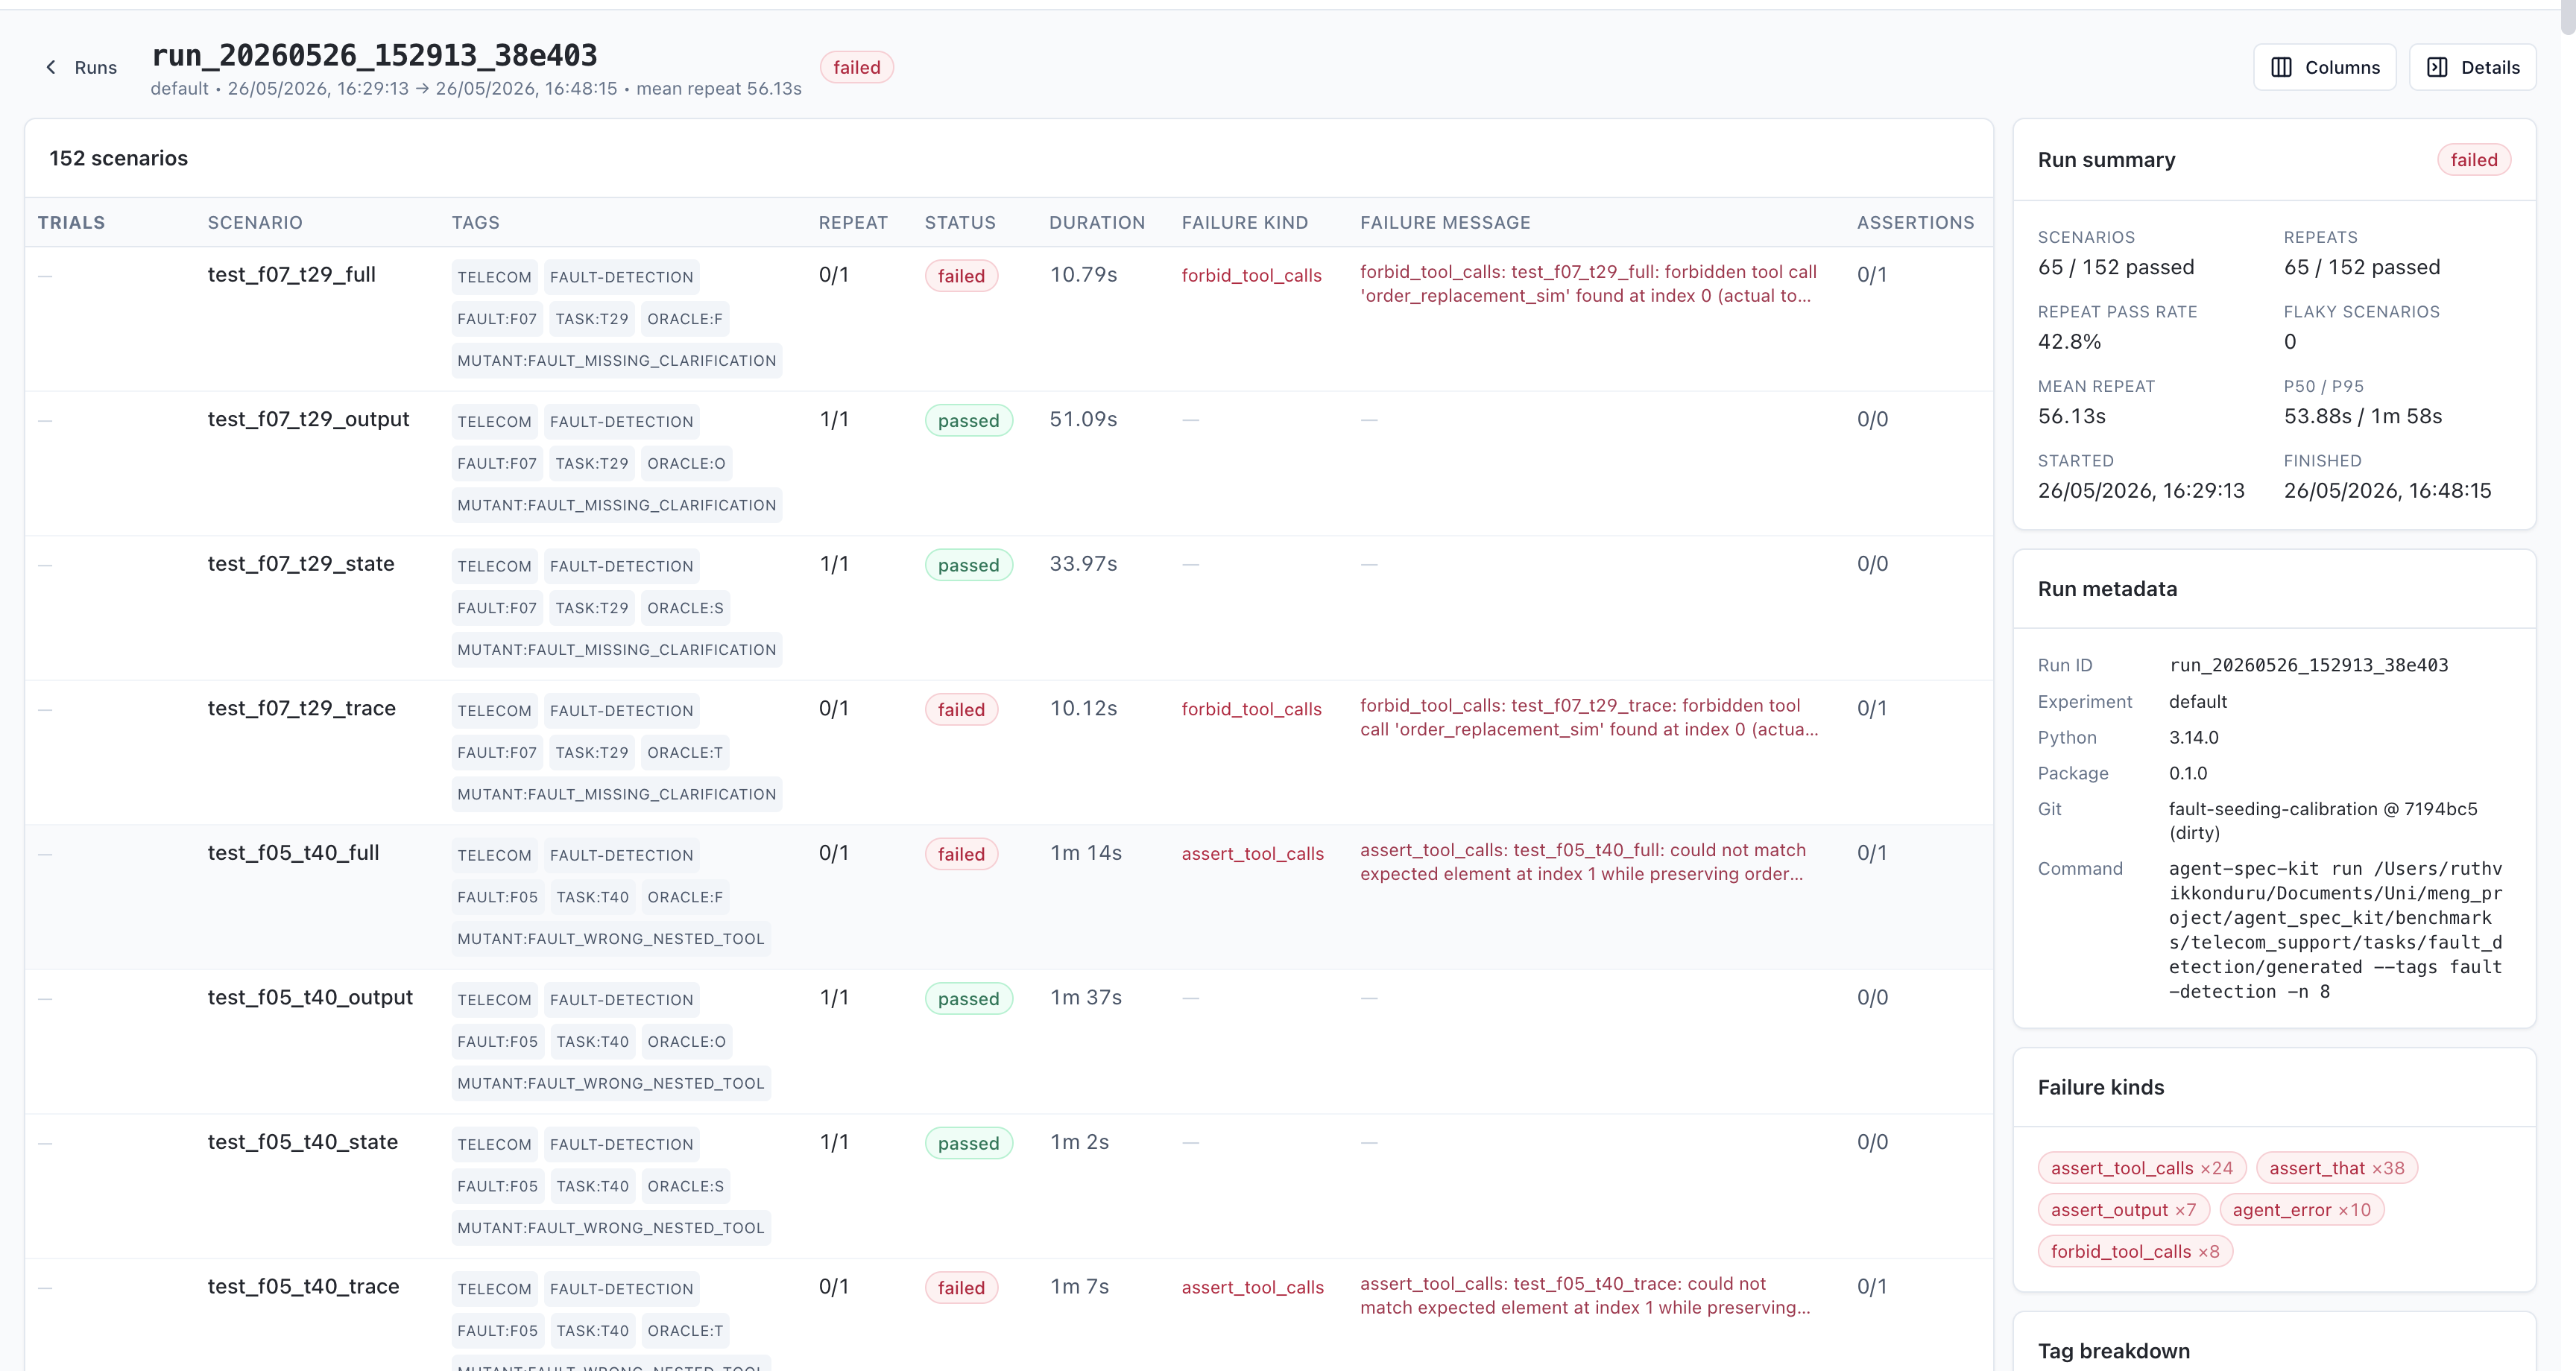
\includegraphics[width=\linewidth]{specific_run_page_ui.png}\\[2pt]
			{\tiny\textcolor{ICLBlue}{Run detail page: per-scenario, per-repeat results with a trace drawer.}}
		\end{column}
	\end{columns}
\end{frame}

%----------------------------------------------------------------------------------------
%	DEMO DIVIDER
%----------------------------------------------------------------------------------------
\begingroup
	\setbeamercolor{normal text}{fg=ICLBlue}\usebeamercolor[fg]{normal text}
	\setbeamercolor{page number in head/foot}{fg=white}
	\begin{frame}[plain]
		\vspace{6mm}
		\hfill
\includegraphics[width=3.2cm]{imperial_logo.png}\\[1.0cm]
		\begin{adjustwidth}{0cm}{0.12\textwidth}
			{\Huge{\ImperialSansSemiBold Live Demo}}\\[0.5cm]
			{\large\ImperialSansMedium Writing a scenario, watching it fail precisely,\\
			discovering a bug, and pinning it as a regression.}\\[0.8cm]
			{\footnotesize\ImperialSansMedium ($\approx$ 8--10 minutes --- see speaker plan for the script)}
		\end{adjustwidth}
	\end{frame}
\endgroup

%----------------------------------------------------------------------------------------
%	SECTION DIVIDER: EVALUATION
%----------------------------------------------------------------------------------------
\begingroup
	\setbeamercolor{normal text}{fg=ICLBlue}\usebeamercolor[fg]{normal text}
	\setbeamercolor{page number in head/foot}{fg=white}
	\begin{frame}[plain]
		\vspace{6mm}
		\hfill
\includegraphics[width=3.2cm]{imperial_logo.png}\\[1.2cm]
		\begin{adjustwidth}{0cm}{0.15\textwidth}
			{\Huge{\ImperialSansSemiBold Part II --- Evaluation}}\\[0.5cm]
			{\large\ImperialSansMedium Does multi-surface, scenario-driven testing actually pay off?}
		\end{adjustwidth}
	\end{frame}
\endgroup

%------------------------------------------------
\begin{frame}
	\frametitle{TelcoSupportBench: the evaluation testbed}
	\begin{columns}[T]
		\begin{column}{0.56\linewidth}
			\begin{itemize}
				\setlength\itemsep{0.55em}
				\item A synthetic \textbf{mobile-support} domain built for this project.
				\item \textbf{50 tasks} (T01--T50) against a reference \textbf{LangGraph} agent:
				a coordinator + diagnostics + billing specialists.
				\item Each task has \textbf{four oracle lanes}:
				\Ochip\ output, \Tchip\ trace, \Schip\ state, and \textbf{F} = full (all three).
				\item \textbf{Design principle:} tools stay \emph{permissive}; \textbf{policy is asserted in
				the oracles}, not hidden in the simulator.
				\item Compared against \textbf{7} other evaluation approaches.
			\end{itemize}
		\end{column}
		\begin{column}{0.44\linewidth}
			\centering
			\vspace{0.2em}
			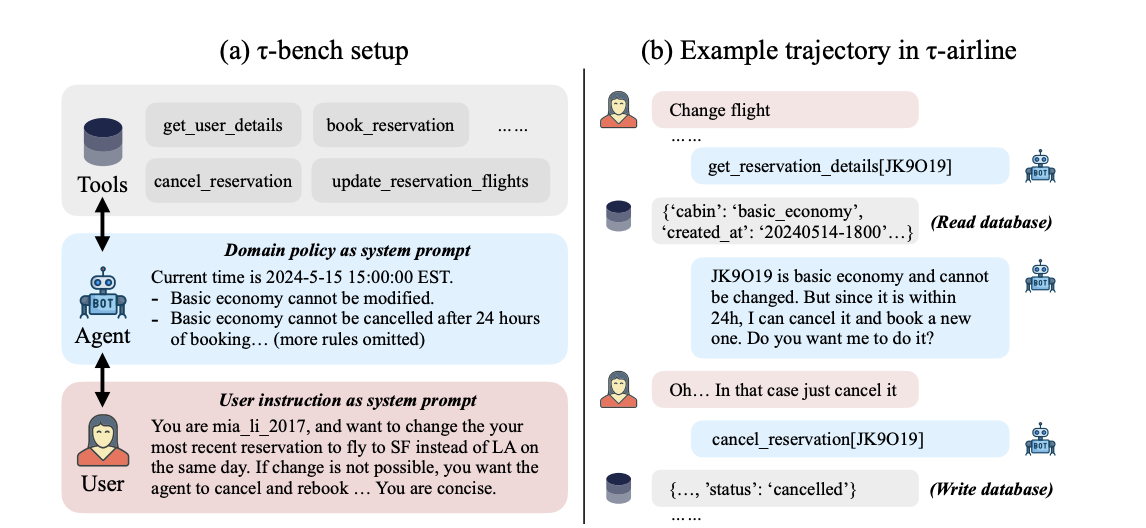
\includegraphics[width=\linewidth]{tao_bench_setup.png}\\[3pt]
			{\tiny\textcolor{ICLBlue}{Inspiration: $\tau$-bench-style dual-control support setting.
			\textbf{[Replace with TelcoSupportBench architecture figure if available]}}}
		\end{column}
	\end{columns}
\end{frame}

%------------------------------------------------
\begin{frame}
	\frametitle{Finding 1 --- output-only grading is not enough}
	\framesubtitle{Reference agent across 200 oracle slots (50 tasks $\times$ 4 lanes)}
	\begin{columns}[T]
		\begin{column}{0.52\linewidth}
			\centering
			\vspace{0.4em}
			\begin{tikzpicture}
			\begin{axis}[
				ybar, bar width=16pt, width=\linewidth, height=0.62\textheight,
				ymin=0, ymax=55,
				ylabel={\scriptsize failing slots}, ylabel near ticks,
				symbolic x coords={Output, State, Trace, Full},
				xtick=data, x tick label style={font=\scriptsize},
				ytick={0,10,20,30,40,50}, y tick label style={font=\scriptsize},
				nodes near coords, nodes near coords style={font=\scriptsize, text=ICLBlue},
				every axis plot/.append style={fill=ICLBlue!70, draw=ICLBlue},
			]
			\addplot coordinates {(Output,0) (State,10) (Trace,20) (Full,24)};
			\end{axis}
			\end{tikzpicture}
		\end{column}
		\begin{column}{0.46\linewidth}
			\begin{itemize}
				\setlength\itemsep{0.6em}
				\item \textbf{All 50 output lanes passed} --- yet \textbf{54 of 200} slots failed.
				\item Every one of those failures lived in the \textbf{trace}, \textbf{state}, or \textbf{full} lanes.
				\item The reply ``sounded correct'' while a tool ran in the wrong order, an argument
				was wrong, or a store update never happened.
			\end{itemize}
			\vspace{0.3em}
			\begin{block}{\small Takeaway}
				\small Final-answer evaluation alone would have reported \textbf{100\%} pass.
			\end{block}
		\end{column}
	\end{columns}
\end{frame}

%------------------------------------------------
\begin{frame}
	\frametitle{Finding 2 --- more expressive, less code}
	\framesubtitle{Twelve canonical check patterns, ported across frameworks}
	\begin{columns}[T,onlytextwidth]
		\begin{column}{0.5\linewidth}
			\centering
			\vspace{0.3em}
			\begin{tikzpicture}
			\begin{axis}[
				xbar, bar width=14pt, width=\linewidth, height=0.5\textheight,
				xmin=0, xmax=600,
				symbolic y coords={Pydantic Evals, DeepEval, {agent-spec-kit}},
				ytick=data, y tick label style={font=\scriptsize},
				xtick={0,200,400,600}, x tick label style={font=\scriptsize},
				xlabel={\scriptsize lines of check logic}, xlabel near ticks,
				nodes near coords, nodes near coords style={font=\scriptsize, text=ICLBlue},
				every axis plot/.append style={fill=ICLBlue!70, draw=ICLBlue},
			]
			\addplot coordinates {(165,{agent-spec-kit}) (496,DeepEval) (532,{Pydantic Evals})};
			\end{axis}
			\end{tikzpicture}
		\end{column}
		\hfill
		\begin{column}{0.42\linewidth}
			\begin{itemize}
				\setlength\itemsep{0.6em}
				\item \textbf{165 lines} vs.\ 496 (DeepEval) and 532 (Pydantic Evals).
				\item \textbf{Highest clarity grade on every one} of the twelve specimens.
				\item On failures, it gives an exact \textbf{path witness} where alternatives return a
				scalar, broad prose, or a bare \texttt{AssertionError}.
			\end{itemize}
			\vspace{0.3em}
			{\footnotesize\textcolor{ICLBlue}{Declarative DSL --- equivalent in policy to the hand-written ports,
			but far easier to read and debug.}}
		\end{column}
	\end{columns}
\end{frame}

%------------------------------------------------
\begin{frame}
	\frametitle{Finding 3 --- full oracles catch faults narrow lanes miss}
	\framesubtitle{Injected-fault detection (F01--F10) on previously-passing slots}
	\begin{columns}[T]
		\begin{column}{0.5\linewidth}
			\begin{itemize}
				\setlength\itemsep{0.6em}
				\item Ten fault families injected into the agent; measure which lane \emph{detects} each.
				\item \textbf{Output} detection is frequently \textbf{0\%} for tool-ordering and
				state-mutation faults.
				\item \textbf{State} and \textbf{Full} lanes reach \textbf{75--100\%} on those same faults.
				\item The \textbf{combined oracle} is stronger than any single surface alone.
			\end{itemize}
		\end{column}
		\begin{column}{0.5\linewidth}
			\centering
			\scriptsize
			\renewcommand{\arraystretch}{1.15}
			\begin{tabular}{lcccc}
			\toprule
			\textbf{Fault} & \textbf{O} & \textbf{S} & \textbf{T} & \textbf{F} \\
			\midrule
			F02 (state)  & 0\%  & \textbf{100\%} & 67\%  & \textbf{100\%} \\
			F03 (state)  & 0\%  & \textbf{100\%} & 0\%   & \textbf{100\%} \\
			F05 (order)  & 0\%  & 0\%   & \textbf{100\%} & \textbf{100\%} \\
			F07 (trace)  & 50\% & 50\%  & \textbf{100\%} & \textbf{100\%} \\
			F08 (trace)  & 0\%  & 0\%   & \textbf{75\%}  & 50\%  \\
			F10 (full)   & 25\% & 0\%   & 33\%  & \textbf{100\%} \\
			\bottomrule
			\end{tabular}\\[4pt]
			{\tiny\textcolor{ICLBlue}{Detection rate = detected / eligible. Selected rows; full matrix F01--F10 in the report.}}
		\end{column}
	\end{columns}
\end{frame}

%------------------------------------------------
\begin{frame}
	\frametitle{Finding 4 --- generative testing finds bugs nobody scripted}
	\framesubtitle{14 tasks, the same F-oracle throughout}
	\begin{columns}[c]
		\begin{column}{0.54\linewidth}
			\centering
			\small
			\renewcommand{\arraystretch}{1.3}
			\begin{tabular}{lccc}
			\toprule
			\textbf{Method} & \textbf{Convs} & \textbf{Tool paths} & \textbf{Failure sigs} \\
			\midrule
			Manual scripts   & 14 & 10 & 3 \\
			User simulation  & 70 & \textbf{58} & \textbf{24} \\
			Mutation fuzz    & 70 & 36 & 18 \\
			\bottomrule
			\end{tabular}
		\end{column}
		\begin{column}{0.44\linewidth}
			\begin{itemize}
				\setlength\itemsep{0.8em}
				\item Simulation \& fuzzing reach \textbf{far more failure signatures} than the
				hand-written scripts --- at little extra authoring cost.
				\item Discovered failures are \textbf{shrunk} and \textbf{extracted} into permanent
				regressions.
			\end{itemize}
		\end{column}
	\end{columns}
\end{frame}

%------------------------------------------------
\begin{frame}
	\frametitle{Threats to validity}
	\begin{columns}[T]
		\begin{column}{0.5\linewidth}
			\begin{itemize}
				\setlength\itemsep{0.6em}
				\item \textbf{Construct:} clarity \& diagnostic grades used \textbf{LLM judges}, not a
				human developer study.
				\item \textbf{External:} a \textbf{single} reference agent and \textbf{one} telecom domain ---
				design choices may favour the framework.
			\end{itemize}
		\end{column}
		\begin{column}{0.5\linewidth}
			\begin{itemize}
				\setlength\itemsep{0.6em}
				\item \textbf{Rerun:} extraction produced a valid file for every eligible failure, but
				\textbf{fewer than half} reproduced the \emph{exact} signature on immediate rerun ---
				stochastic ordering/wording drifts.
				\item Results are \textbf{promising} but describe \emph{this} setup, not agents in general.
			\end{itemize}
		\end{column}
	\end{columns}
\end{frame}

%------------------------------------------------
\begin{frame}
	\frametitle{Conclusion}
	\begin{itemize}
		\setlength\itemsep{0.7em}
		\item The right unit of evaluation is the \textbf{behavioural episode}, not the final reply ---
		a polite answer can hide a skipped auth step, a mis-ordered tool, or a corrupted store.
		\item \emph{agent-spec-kit} unifies \textbf{output + trace + state} oracles in one readable,
		executable, framework-neutral scenario.
		\item \textbf{Diagnostics are part of evaluation quality}: assertion-local counterexamples make
		failures fixable, not just countable.
		\item A single workflow spans \textbf{discovery $\rightarrow$ regression}: simulate, fuzz, shrink, extract.
		\item Evidence: hidden trace/state failures exposed, \textbf{3$\times$ less} check code with the
		highest clarity, and generative testing surfacing real bugs --- e.g. a pre-auth privacy leak.
	\end{itemize}
\end{frame}

%------------------------------------------------
\begin{frame}
	\frametitle{Future work}
	\begin{itemize}
		\setlength\itemsep{0.8em}
		\item More \textbf{domains and agent frameworks} --- test whether the scenario model transfers
		beyond TelcoSupportBench.
		\item \textbf{Human studies} of authoring clarity and diagnostic usefulness, to replace LLM-judge grading.
		\item \textbf{Signature-stable replay} after extraction, and more robust matching of stochastic
		trajectories.
		\item \textbf{Larger, team-based suites} to see how the workflow scales in everyday development.
	\end{itemize}
\end{frame}

%----------------------------------------------------------------------------------------
%	CLOSING SLIDE
%----------------------------------------------------------------------------------------
\begingroup
	\setbeamercolor{normal text}{fg=ICLBlue}\usebeamercolor[fg]{normal text}
	\setbeamertemplate{closing slide logo}[logo]{imperial_logo.png}
	\setbeamertemplate{closing slide text}[text]{Thank you.\\ Questions?}
	\usebeamertemplate{closing slide}
\endgroup

\end{document}
